\documentclass[AMA,LATO1COL]{WileyNJD-v2}

\usepackage[english]{babel}
\usepackage[utf8]{inputenc}
\usepackage{cite}
\usepackage{amsmath,amssymb,amsfonts}
\usepackage{graphicx}
\usepackage{subcaption}
\usepackage{textcomp}
\usepackage{xcolor}
\usepackage{url}
\usepackage{xspace}
\usepackage{todonotes}[disable]
\newcommand{\comment}[1]{\todo[color=yellow!40, inline]{\footnotesize{#1}}}
\newcommand{\henrique}[1]{\todo[color=blue!40, inline]{\footnotesize{Henrique: #1 }}}
\newcommand{\keerthana}[1]{\todo[color=pink!40, inline]{\footnotesize{Keerthana: #1 }}}
\newcommand{\serge}[1]{\todo[color=orange!40, inline]{\footnotesize{Serge: #1}}}
\newcommand{\review}[1]{\todo[color=green!40, inline]{\footnotesize{Reviewer: #1}}}

\newcommand{\challengecount}[0]{\textsc{18}\xspace}
\newcommand{\techcount}[0]{\textsc{44}\xspace}
\newcommand{\techgroupcount}[0]{\textsc{6}\xspace}


\articletype{Special Issue Paper - Perspective}%

\received{31 July 2021}
\revised{day month year}
\accepted{day month year}

\raggedbottom

\begin{document}

\title{Systematic Literature Review on Microservices: \\ Challenges and Technologies}

\author[1]{Keerthana Sanala Prakash}

\author[2]{Henrique Rocha}

\author[3]{Marco Túlio Valente}

\author[1]{Serge Demeyer}

\authormark{Prakash \textsc{et al}}


\address[1]{\orgdiv{Department of Computer Science}, \orgname{University of Antwerp}, \orgaddress{\country{Belgium}}}

\address[2]{\orgdiv{Department of Computer Science}, \orgname{Loyola University Maryland}, \orgaddress{\country{USA}}}

\address[3]{\orgdiv{Deparment of Computer Science}, \orgname{UFMG}, \orgaddress{\country{Brazil}}}

\corres{Henrique Rocha. \email{henrique.rocha@gmail.com}}

%\presentaddress{This is sample for present address text this is sample for present address text}

\abstract[Summary]{As microservice architecture is a new research area, the need for a systematic literature review is important to summarise the state of the art and identify the potential for future studies. Although various studies have been conducted which cover the microservice challenges, it is still strenuous to get a clear image of all the existing challenges one needs to understand while adopting microservices. In this paper, we conducted a systematic literature review to understand the challenges in adopting microservices and the technologies used in implementing microservices.
In our systematic literature review, we collected 81 primary studies. We identified that the most common challenges in adopting microservices are migration (14 references), performance (11 references), scalability (10 references), and testing (10 references). For the technologies used in implementing microservices, container technologies (i.e., docker, kubernetes) are the most cited (14 references). Moreover, the second most cited are the programming languages and Other technologies used to develop microservices (13 references). The resulting study can serve as a foundation for researchers and practitioners to plan and implement microservices.
}

\keywords{microservices, systematic literature review, service oriented architecture, internet of things.}

\jnlcitation{\cname{
\author{Prakash K}, 
\author{Rocha H}, 
\author{Valente M.T}, and 
\author{Demeyer S}} (\cyear{2021}), 
\ctitle{Systematic Literature Review on Microservices: Challenges and Technologies}, \cjournal{J Softw Evol Proc}, \cvol{2021;00:X--Y}.}

\maketitle

%\footnotetext{\textbf{Abbreviations:} ANA, anti-nuclear antibodies; APC, antigen-presenting cells; IRF, interferon regulatory factor}


% !TEX root = ../2021_microservices_wileytemplate.tex

\section{Introduction}

During the last ten years, cloud computing, and the relatively low cost of server renting services like amazon web services, azure, and google cloud have opened the opportunity to build businesses around cloud technologies. This model also brings new challenges to scale and maintain systems.\cite{Claus2016} Inspired by service-oriented computing, microservices are small applications with a single responsibility that can be deployed, scaled, and tested independently. The concept was created as service-oriented architecture (SOA) 10 years back. It is about fragmenting complex applications into small pieces and a fluid delivery model that delivers services on demand, thus improving performance.\cite{Larrucea2018}

Microservices are an architectural style that structures an application as a collection of independent modules. These modules are highly maintainable, testable, loosely coupled, independently deployable, and each isolates a functionality. Therefore, we can split the application into distinct independent services~\cite{thones2015}. Recently, microservice architecture became a strategic solution for decomposing large monolithic applications into smaller manageable services.\cite{Taibi2019} 
%In microservices, every application function is its service, own container, and communicate via Application programming interface (API)~\cite{Danbettinger2019}.

For several years, monolithic architecture was the widely-used architecture for building web and mobile applications. The server-side system is based on a single application and is easy to develop, deploy, and manage.\cite{Danbettinger2019} The advantage is that if we want to change functionalities, it is enough to implement these changes in one place architecture-wise.\cite{Pavlovic2020} Single point of failure, technology lock-in, and limited scalability are a few other drawbacks of monolithic applications. Growing companies are considering other architecture styles such as microservices.\cite{Lenga2019, Jag2017, Rodrigue2016}

The design, development, and operation of microservices are picking up more momentum in the industry. At the same time, academic work on the topic is at an early stage.\cite{Soldani2018, Dragoni2017, Olaf2016} 
Companies are working day-by-day on the practical implementation of microservices.\cite{Kevin2015, Alpers2015} For instance, the microservices architecture allowed netflix\cite{Meshenberg2016} to greatly speed up the development and deployment of its platform and services.

The academia is joining microservices architectural patterns to other disciplines. For example, devOps and internet of things (IoT)\cite{Osses2019}. However, there is still no clear perspective of emerging recurrent solutions or design decisions in microservices both in industry and academia.\cite{Soldani2018} Despite the hype for microservices, both industry and academia still lack consensus on the adequate conditions to embrace and benefit from this new paradigm.\cite{Dragoni2017} It also brings new challenges in scaling and maintaining the system as fast as we are moving towards using a microservices architecture.

While many organizations like Netflix,\cite{Meshenberg2016} Uber,\cite{Uber} and Amazon\cite{Amazon} have proposed solutions to certain challenges, they focus only on their organizational perspective. It is also suggested that every challenge is tailored for each company and the solutions proposed by one may not be well-suited to others.\cite{Kevin2015} Many aspects of the practical challenges in microservices are still unexplored. This makes it difficult for researchers or practitioners to know where to start the adoption process. The goal of this paper is to characterize the possible overall challenges faced when adopting microservices and technologies involved in microservice implementation. To achieve this goal, we conducted a systematic literature review.\cite{Kitchenham2007} More specifically, we designed two research questions, the first one related to the challenges and the second to technology solutions in implementing microservice, to guide our literature review. 
%
The main contribution of the paper includes the recent challenges after the introduction of microservice and a list of technologies that have been used in leveraging the implementation of microservice. We also discuss proposed solutions we found in the literature to address the main challenges.

The rest of the paper is structured as follows. *** Revise the Sections later *** In Section~\ref{sec:background}, we describe background information on microservice and monolith; we also explain the importance to migrate from monolith to microservices. In Section~\ref{sec:study-design}, we describe the method and protocol followed in our systematic literature review. In Section~\ref{sec:results}, we answer the research questions and cover the challenges and technologies used in microservice. In Section~\ref{sec:discussion}, we discuss possible solutions for challenges mentioned in the studied literature. In Section~\ref{sec:threats}, we cover the threats to the validity of our study. In Section~\ref{sec:related-work}, we present the related work. Finally, in Section~\ref{sec:conclusion}, we conclude the paper and outline future work ideas.





%% !TEX root = ../final_paper.tex

\section{Background}\label{sec:background}

\par Microservices are an architectural style that structures an application as a collection of independent modules. These modules are highly maintainable, testable, loosely coupled, independently deployable, and each isolates a functionality. Therefore, we can split the application into distinct independent services~\cite{thones2015}. Recently, microservice architecture has evolved as a paradigm shift in decomposing large monolithic applications into smaller manageable services with their code base and deployment infrastructure~\cite{Taibi2019}. In microservices, every application function is its service, own container, and communicate via Application programming interface (API)~\cite{Danbettinger2019}.

\par We can describe microservices as simple and stateless. In a microservices world, business requirements are divided into independent features and each of them is built as an individual service when deployed in separate containers. Therefore, it is easy to build and deploy, especially when it is containerized~\cite{Pavlovic2020, Zaytev2018}. Microservices are loosely coupled because they can be developed and released independently of each other. Since services interact over technology-agnostic protocols like HTTP, services could use any technology~\cite{Jaleel2017}. Microservices bring many benefits to applications. Although, service level independent scalability has been considered as the most value-adding advantage for choosing microservices architecture for applications.

\par For several years, a monolithic architecture was the widely-used architecture for building web and mobile applications. The server-side system is based on a single application and easy to develop, deploy, and manage~\cite{Danbettinger2019}. These applications are mostly characterized by individual programs handling multiple functionalities~\cite{Francesco2019}. They often have one database that is shared by all departments. This has the advantage that if we want to make a change in all services, it is enough to implement this change in one place~\cite{Pavlovic2020}. It is this simplicity at the start that seems to be the greatest advantage of monoliths. We do not have to think about the division of services and functions. Though monolithic applications are known to be easier to operate, as the systems grew bigger, they also increased the complexity for coding, deployment, and maintenance stages of the software development life cycle~\cite{Kalske2017, Santos2020}. Single point of failure, technology lock-in, and limited scalability are a few other drawbacks of monolithic applications. Growing companies are considering other architecture styles such as microservices~\cite{Lenga2019, Jag2017, Rodrigue2016}. The most common reasons teams migrate to microservices are resilenced and continuous delivery, amongst other challenges~\cite{haugeland2020}.


\par Adopting microservices comes with a cost~\cite{villamizar2017} at the information technology (IT) operational level because of the expenses incurred for deployment, load balancing, process monitoring, and scalability for each service. If not adopted well, one might end up having technical debt. On the other hand, container platforms like docker and kubernetes provide these functions as part of their features~\cite{Sharaf2019, Venugopal2017}. These platforms help in scalability, making it the compelling architecture choice for applications.

\par Microservices use http as the protocol for synchronous communication and multiple service endpoints may give malicious attackers more opportunities for system penetration. Hence, it is important to secure microservices-based applications with proper authentication and authorization methods~\cite{Jaleel2017, Dragoni2017}.




%% !TEX root = ../2021_microservices_wileytemplate.tex

\section{Study Design}\label{sec:study-design}

We conducted a systematic literature review (SLR) conforming to the guidelines presented by Kitchenham and Charters.\cite{Kitchenham2007} A systematic literature review (SLR) is a method of reviewing data and results from research about a particular question in a standardized systematic way.\cite{Sebastian2018} According to Garousi et al.,\cite{Garousi2016} it is important to complement scientific papers in an systematic literature review by also analyzing grey literature. Therefore, we decided to adapt our systematic literature review protocol to include grey references.
%
In this section, we describe the designed protocol for our systematic literature review which was enhanced with grey literature. We divided our protocol into the following steps: (1) Background, (2) Research questions, (3) Search procedure, (4) Selection criteria, (5) Grey literature, and (6) Data extraction and synthesis.

\subsection{Background}

After we defined the protocol, we started by reading papers to understand the current scope of microservices research. 
%
The first papers we study were a systematic literature review\cite{Ghani2019} and systematic mapping studies\cite{Claus2016, Francesco2019} since both types provide an overview of the state of the art on microservices. Then, we performed a backwards snowballing procedure to gather more references for this initial knowledge on microservices research.\cite{Larrucea2018, Soldani2018, Dragoni2017, Olaf2016, Kevin2015, Meshenberg2016, Osses2019, ghofrani2018, Shady2020, Michael2018, Toledo2019, Matt2016}

Based on the studied references, we developed the rationale for this study (Sections I and II). Moreover, with an understanding of the research state-of-the-art, we were prepared to elaborate the research questions we aimed to investigate. 

\subsection{Research Questions}

The leading goal of this research is to analyze the possible challenges in adopting microservices. Moreover, we have also deemed it important to cover the technologies used in implementing microservices and solving such challenges. Therefore, we elaborated the following research questions to guide our systematic literature review:

\begin{itemize}
  \item RQ\#1: What are the main challenges when adopting microservices?
  \item RQ\#2: What are the main technologies used for implementing microservices?
\end{itemize}


\subsection{Search Procedure}

%This step describes the search procedure we followed to acquire scientific references. 
We planned our procedure to search for microservices papers that would discuss challenges and technologies (i.e., tackle our research questions) but without biasing the search results. 
We performed a manual search using google scholar as the search engine. 
We chose google scholar because it combines results from multiple digital libraries. 
%We excluded citations and patents from the search.

We developed a strategy to choose the appropriate search string for our research. Two authors proposed candidate strings and analyzed if the top results seem relevant for our research. We also needed a string that would not give too many results for the authors to handle manually. Therefore, the total number of results was also a factor in choosing the string. Moreover, we did not want the search string to be biased. After one week of analyzing candidate strings, we settled on the following: \texttt{microservices "architecture style" design}. The chosen string produced 471 references at the time we collected its results (2020-11-12). 
%Figure~\ref{fig:total-papers-per-year} shows the search results divided per year.

%\begin{figure}[h]
%	\centering
%	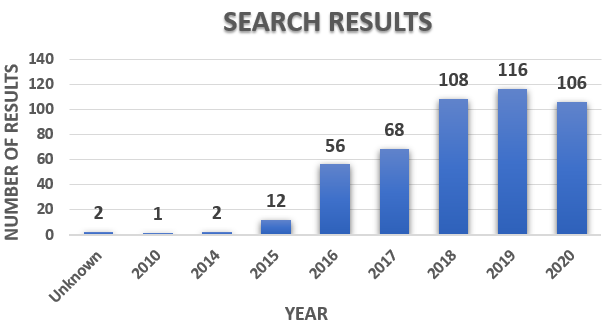
\includegraphics[width=0.5\linewidth]{images/yearvsarticles.png}
%	\caption{Search results per year before applying the selection criteria.}
%	\label{fig:total-papers-per-year}
%\end{figure}	 


\subsection{Selection Criteria}

Selection criteria determine which studies to include or exclude from a systematic literature review. 
Since the search provided a good amount of results, we focused on defining rejection criteria to exclude irrelevant results as follows:
%Our selection criteria are detailed as follows:
%Table~\ref{tab:selection-criteria} summarizes our selection criteria which we detail as follows:

%\begin{table}[h]
%\centering
%\caption{Selection Criteria}
%\label{tab:selection-criteria}
%\begin{tabular}{|l|p{5cm}|}
%\hline
%	& \\
%	& R1: Duplicate papers \\
%  	& R2: Not written in English \\
%   	& R3: Not peer-reviewed \\
%Exclusion Criteria    
%	& R4: Published before 2017 \\
%   	& R5: Select Extended versions \\
%   	& R6: Unrelated based on title \\
%   	& R7: Unrelated based on abstract  \\
%   	& \\
%\hline
%\end{tabular}
%\end{table}


\begin{itemize}
   \item \textbf{R1: Duplicated papers.} The search engine we used acquires papers from multiple libraries. Therefore, the results can contain the same paper more than once but from different sources. %Then, we reject all duplicated instances of a paper that is already in our study.
   \item \textbf{R2: Not written in English.} A paper can have an English abstract and keywords even though the paper content is written in another language. The search engine may still present such papers based on their abstracts.
  \item \textbf{R3: Not peer-reviewed.} Some digital libraries allow users to post papers that were not peer-reviewed. Since the selection criteria are to choose scientific papers,  peer-review is very important to maintain academic integrity. %We rejected all papers that were not peer-reviewed.
   \item \textbf{R4: Publication from 2017 to 2020.} 
%We exclude papers published before 2017. 
We wanted this study to focus on the most recent studies on microservices.
  \item \textbf{R5: Multiple versions.} When a paper has multiple versions of itself, we reject the previous versions and keep only the most current one. For example, if a paper published on a conference is later extended to a journal paper, we would reject the conference version and keep the journal as it is the most current.
  \item \textbf{R6: Unrelated based on title.} For this criterion, we read the title of the paper to assess if it was indeed a relevant study to answer our research questions. The titles deemed unrelated were excluded.
  \item \textbf{R7: Unrelated based on abstract.} For this criterion, we read the abstract of the paper to verify if it would help to answer our research questions. The abstracts that were not related to our research were rejected.  
\end{itemize}


We apply the selection criteria in the same order as shown, i.e., we apply R1 first then followed by R2, and so forth.
From the described selection criteria, only the last two (R6 and R7) are subjective. To mitigate the subjectiveness of such criteria, we had two persons (the first and second authors) working separately to review them. In case of disagreement, the paper would be included in study. Therefore, we only rejected papers if both persons marked it as unrelated.

As we previously described, the search returned a total of 471 results. After applying our selection criteria, we obtained 60 studies (i.e., 311 papers were rejected). Figure~\ref{fig:selection-criteria} shows the number of papers rejected by each criterion, and 'A' marks the total of accepted papers after the rejection criteria were applied.

%The selection criteria are used to determine which studies could be included and excluded as shown in table 1. We analyze the data on the specific questions and which are most relevant to the answer the questions. Below table 1 shows the inclusion, exclusion criteria as determined from the research questions generated after the selection of the primary study. A study will be disqualified if it meets any of the following exclusion criteria. The study selection criterion has two major phases. In the first phase, the study inclusion/exclusion steps were applied as shown from i1 to i4 and R1 to R5. In the second phase, the study screening criterion was applied to the Title and Abstract. In both of the phases, the focus of the study is on microservices, and the existence of empirical work was ensured. As a result of the first screening phase (Title and Abstract screening), we obtained 471 studies as shown in figure 1. These 471 studies were screened for full-text inclusion/exclusion in the second phase. After applying inclusion/exclusion criteria to the full text we obtained 60 studies. In figure 2, the Exclusion criteria stepwise study screening process count is shown along with the number of studies excluded after each screening step. 

\begin{figure}[h]
	\centering
	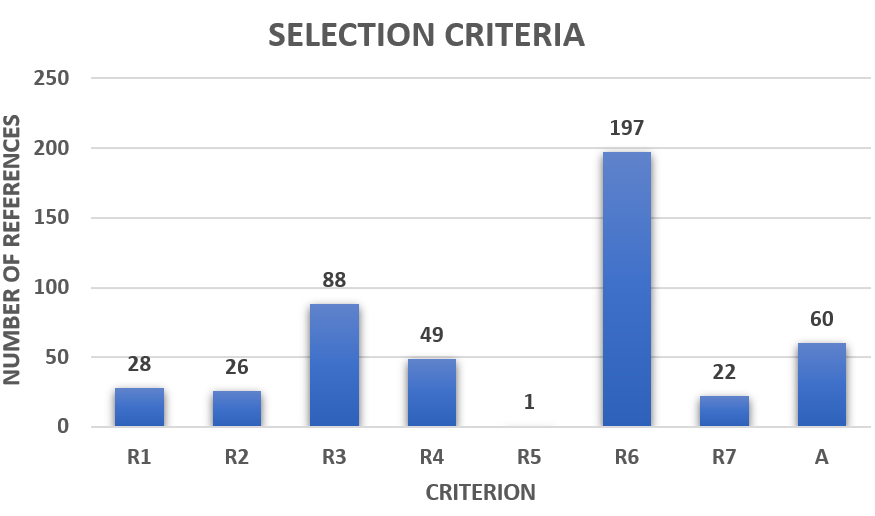
\includegraphics[width=0.5\linewidth]{images/exclusion.png}
	\caption{Selection criteria showing the number of scientific references rejected by each exclusion criterion (R1 to R7) and the number of accepted (A) references.}
	\label{fig:selection-criteria} %%Do not put spaces in the label name, and try to use a name easier to relate to the figure
\end{figure}	


\subsection{Grey Literature}

We decided to complement the scientific references that passed our selection criteria with grey literature.\cite{Garousi2016} Since microservices is a popular topic amongst practitioners, we believe it is important to include their knowledge in our research. The use of grey literature can serve as evidence of practitioners' knowledge and experience.\cite{Kamei2019}

Intended as materials and research studies produced outside at the organization of traditional commercial and academic is important. grey literature publications include news, blogs, videos, etc. However, grey literature could be of a risk that there might be no technical evidence or evaluation. Although for the scope of this study, we tried to include legitimate speakers and bloggers from companies.
%
For this study, we started by collecting videos from the goto conference$^\dagger$\let\thefootnote\relax\footnote{$\dagger$ \url{http://gotocon.com/aboutjaoo/}} which is an event for practitioners. Then we searched for microservices content by respectable sources. 

Guidelines for grey literature review\cite{Garousi2019} state it is important to define stop criteria when gathering grey literature sources. One of the reasons for stopping rules is the large volume of data one can encounter when searching for grey literature.\cite{Garousi2019}

We decided to set our stop criteria when our grey reference numbers achieved more than one-third of the scientific references we selected in the previous phase, i.e., 21 references$^\ddagger$\let\thefootnote\relax\footnote{$\ddagger$ We collected 60 scientific references in the previous step. Therefore, one-third of 60 would be 20 references. Since we defined our criterion to be more than one-third (instead of exactly one-third), we needed at least one more reference.} in total. Therefore, we collected 21 references from grey sources.
%
The 21 grey literature references were added to our 60 scientific references, for a total of 81 references. %(Figure~\ref{fig:stats-total}). 
%In the next steps of the protocol, we use the total references from both scientific and grey literature.

%\begin{figure}[h]
%	\centering
%	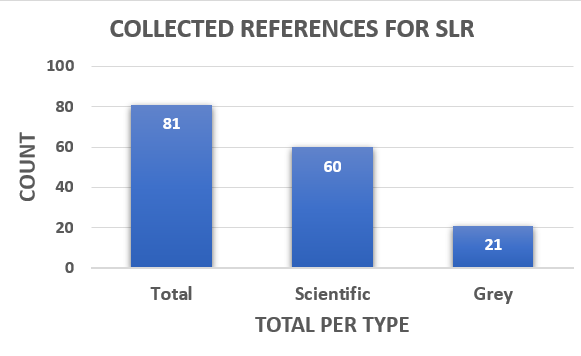
\includegraphics[width=0.5\linewidth]{images/stats_total}	
%	\caption{Total number of collected references used in our systematic literature review (SLR).}
%	\label{fig:stats-total}
%\end{figure}		


\subsection{Data Extraction and Synthesis}

For the data extraction procedure, we read all the 81 papers that we collected. For each paper, we focused on understanding and cataloging information that would address our research questions. We categorized the extracted information and stored it on a spreadsheet for easy access. 

More specifically, the data extraction scheme had three main constituents. First, we extracted data about general information of the publication. Second, we extracted data for RQ\#1 and then for RQ\#2. Data for RQ\#1 is specifically related to all the challenges in adopting microservices. Data extracted for RQ\#2 is about the technologies which are used in implementing the microservices and solutions to the challenges are explained in the discussion (Section~\ref{sec:discussion}).
%
By the end of the extraction process, we identified \challengecount distinct categories related to challenges (i.e., RQ\#1), and \techcount different technologies which we grouped into \techgroupcount major categories (i.e., RQ\#2). 
%Our spreadsheet containing the full extracted data is publicly available on our website.\footnote{\url{https://uantwerpen-my.sharepoint.com/:x:/r/personal/s0160228_ad_ua_ac_be/_layouts/15/Doc.aspx?sourcedoc=%7BAA565D3C-022C-4E29-A968-180B213934BA%7D&file=Data_collection.xlsx&action=default&mobileredirect=true}} 

%\subsection{Data Synthesis}

For the synthesis, we grouped the categories we extracted from the data extraction into another spreadsheet. That way, we have condensed information where the challenges and technologies/solutions are the main protagonist. For instance, by using this spreadsheet, we can easily find which papers presented a particular challenge. 
%
%We present the outcomes and findings of the synthesized data in Section~\ref{sec:results}.




%% !TEX root = ../2021_microservices_wileytemplate.tex

\section{Results}\label{sec:results}

In this section, we present the results from our systematic literature review. First, we show a general overview of the collected paper's characteristics (Section~\ref{sec:results-general}). Then, we present our results to answer our first research question related to challenges (Section~\ref{sec:results-rq1}). Finally, we describe our findings to answer our second question on the topic of technologies (Section~\ref{sec:results-rq2}).

\subsection{General Analysis}\label{sec:results-general}

Figure~\ref{fig:collected-papers-slr} shows an overview of the collected literature references we used in our systematic literature review. In our study, we have a total of 81 references, of which 60 are from scientific sources and 21 come from grey literature. 

\begin{figure*}[h]
    \centering
    \begin{subfigure}[b]{0.40\textwidth}
        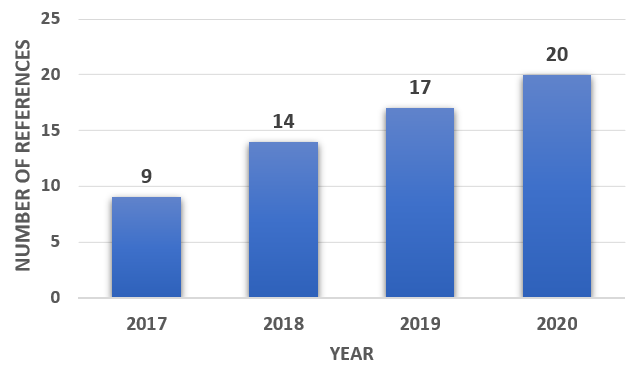
\includegraphics[width=\textwidth]{images/publicationtypes_1.png}
        \caption{Scientific references per year}
        \label{fig:papers-academic-year}
    \end{subfigure}
~
    \begin{subfigure}[b]{0.25\textwidth}
        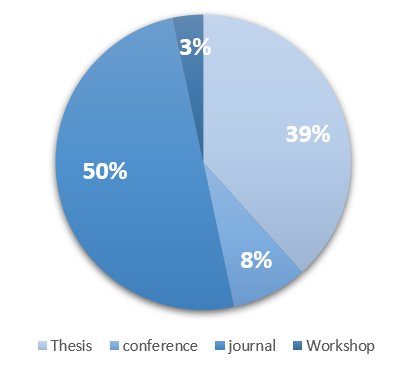
\includegraphics[height=0.2\textheight]{images/publicationtypes_3.png}
        \caption{Types of the scientific references}
        \label{fig:papers-academic-type}
    \end{subfigure}

    \begin{subfigure}[b]{0.40\textwidth}
        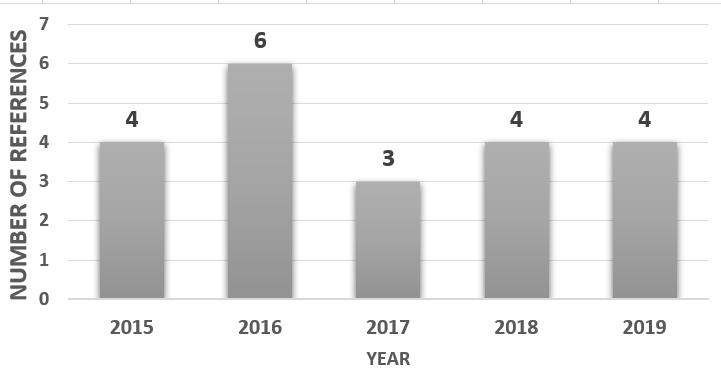
\includegraphics[width=\textwidth]{images/greytype_1.png}
        \caption{Grey references per year}
        \label{fig:papers-grey-year}
    \end{subfigure}
~
    \begin{subfigure}[b]{0.25\textwidth}
        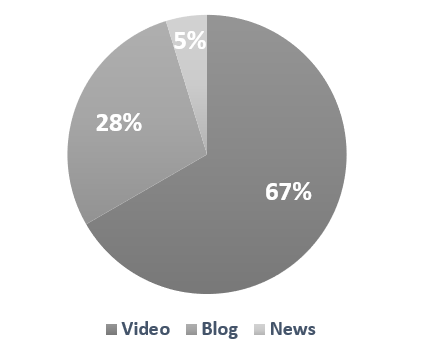
\includegraphics[height=0.2\textheight]{images/greytype_2.png}
        \caption{Types of the grey references}
        \label{fig:papers-grey-type}
    \end{subfigure}

    \caption{collected references Used in the systematic literature Review}\label{fig:collected-papers-slr}

\end{figure*}


We can see the number of scientific references we deemed relevant for our study to grow each year after 2017 (Figure~\ref{fig:papers-academic-year}). Even though we reject papers from before 2017 from our study, we did not design our remaining selection criteria to favor more current papers. Therefore, the rise in the number of references per year is probably just a coincidence. 
%In Figure~\ref{fig:selected-papers-slr-1} We can see the number of papers published after 2017 and the number is growing more every year. In Figure~\ref{fig:selected-papers-slr-2} We can see here the types of publications collected during the SLR \henrique{These are questionable remarks. Since you selected these papers, you cannot claim a generalized trend or a raise.}\keerthana{fixed it}
%
On the other hand, most of the grey literature we used in this study is from 2016 (Figure~\ref{fig:papers-grey-year}). The reason is that the goto conference was our initial starting point to collected grey references. Particularly in 2016, many speakers were discussing microservices in the goto conference.

When we look at the types of literature, we have different classifications for scientific (Figure~\ref{fig:papers-academic-type}) and grey (Figure~\ref{fig:papers-grey-type}). Since all scientific references were papers, we classified them by their publication type (e.g., journal paper, conference paper, thesis). For grey, we classified the references by their media type and publishing format (e.g., video, blog). 
%
%Figure~\ref{fig:selected-papers-grey-1} shows the types of grey literature collected year-wise. There was a total of 21 grey literature which includes blogs, Youtube videos, and News. We could see that there was a lot of grey literature initially published and this serves as a key for practitioners or academia to learn from it and start making more grey literature.
%
From the selected references, we could see there is a good variety of publications. %This may indicate that microservices are discussed in many fields for both the industrial and academia.


\subsection{RQ\#1: What are the main challenges when adopting microservices?}\label{sec:results-rq1}

\begin{figure*}[t]
	\centering
	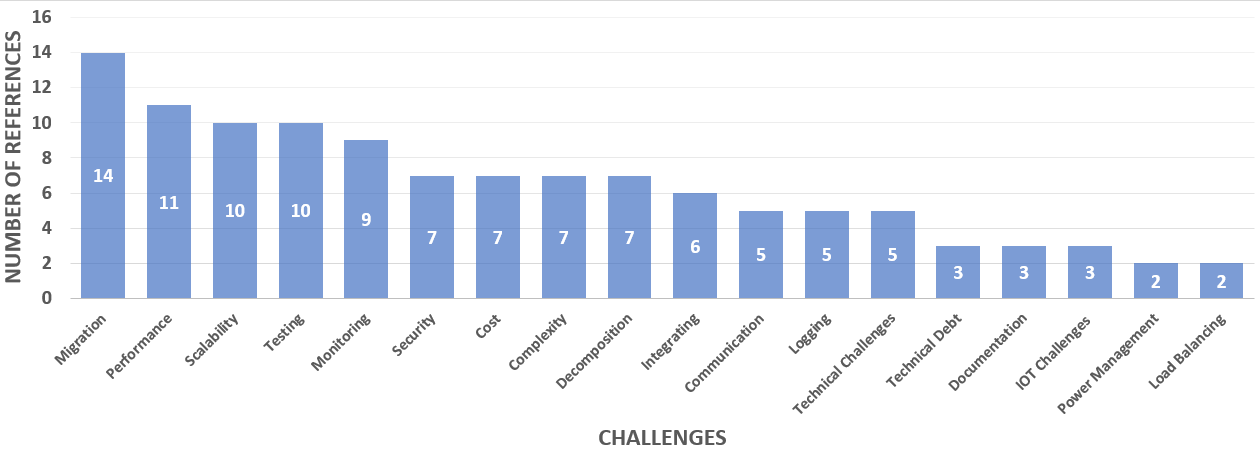
\includegraphics[width=0.9\linewidth]{images/Challenges_updated.png}
	\caption{Challenges in adopting microservices }
	\label{fig:challenges}
\end{figure*}	

In this section, we answer our first research question by analyzing the collected data.
To answer RQ\#1, we examined the spreadsheets created in the data synthesis phase from our 81 references.

Figure~\ref{fig:challenges} shows the challenges in adopting microservices that we discovered in our systematic literature review. It also shows how many distinct references in our selection discuss such challenges. 
According to our classification, we identified \challengecount challenges.
The challenges mentioned on the most number of references are migration and performance, followed by scalability and testing. In our collected data, those are the major challenges of adopting microservices.


\subsubsection{Migration}%#1
When migrating an application the {codebase update~\footnote{Before undertaking any major structural changes, the codebase would have to be updated and unified to make any further changes easier. The technical problems of the outdated codebase, the difficulty of adding new features, and the inferior performance of parts of the application would be targeted}} are difficult tasks as observed from the publication by Tuuli and Wang~\cite{Tuuli2020, wang2020}. 

Database migration is the main problem and risks if the application has a database, and especially its location inside the application docker container. To ensure the stability and maintainability of the application database, it would have to be migrated from its current location to a better alternative ~\cite{Tuuli2020}.

\par Hosting service migration is seen as the main problem in focus during this step were the uneven server load, as well as the difficulty of applying updates to the application~\cite{Tuuli2020}. Many organizations are planning and migrating their on-premise software to the cloud, starting with the Infrastructure as a service (IaaS) and Software as a service (SaaS) models. Nonetheless, they are facing some challenges and difficulties, mainly in the Platform as a service (PaaS) model, related to the complexity in integrating the legacy and internal systems~\cite{rosa2018}. It requires a different way of thinking compared to the traditional way of software architectures, often leading to the migrations and creations of these architectures being long and costly processes~\cite{leo2019}.
\par System application migration is becoming an emerging issue with different challenges. Migration of the system to microservice optimizes decentralization, replaceability, and autonomy of software architectures. Although researchers are not convinced of any specific definition of microservice, its modeling techniques, and its properties, it is aware of system migration to microservices~\cite{ghayyur2018}.
\par Migration of the resulting application towards the new intended state is still a (partially) manual and labor-intensive step~\cite{overeem2018}. If on the one hand microservices can help in achieving a good level of flexibility (e.g., by promoting low services coupling, higher maintainability), on the other hand adopting a microservice-based architecture may bring higher complexity~\cite{Difrancesco2017}. The microservice architectural style has become an essential element for the development of applications deployed on the cloud and for those adopting the devops practices. Nevertheless, while microservices can be used to develop new applications, there are monolithic ones, that are not well adapted neither to the cloud nor to devops. Migrating these applications towards microservices appears as a solution to adapt them to both. 


\par Companies have been widely investing in modernizing the software architecture and development processes of their products. By migrating away from software monoliths towards the emerging microservice architecture style, an agile and robust software system with a compatible development process can be accomplished. Despite this, modernization can be highly challenging from a practical point of view. Available software solutions, which aim at supporting the restructuring of software monoliths into microservices, often do not satisfy the arising demands of the developers. While these products offer diverse static analysis functionalities, dynamic analysis aspects are mostly missing. Yet, especially a dynamic analysis can provide invaluable information about overlooked characteristics of the software system~\cite{Lenga2019}.

\par Serious efforts have been undertaken to move from monolithic architectures to microservice architectures. The common problem in these efforts is to identify from monolithic applications the candidates of microservices which includes the programs or data that can be turned into cohesive, standalone services; this is a tiresome manual effort that requires analyzing many dimensions of software architecture views and often heavily relies on the experience and expertise of the expert performing the extraction~\cite{Kamimura2018}\cite{selmadji2020}.

\subsubsection{Performance}%#2

Goldsmith~\cite{Kevin2015} talks about challenges related to monitoring, latency, and problems with completely autonomous teams. The distributed aspect of a microservice system is a significant challenges~\cite{Matt2016}. Its distributed nature impacts the performance of the system. Calls to a single service might trigger a cascade of additional calls to other services distributed across a network, each adding its latency. The increase in resource usage may cause a microservices-based application to execute slower~\cite{Etsy, Netflix}. It can be hard to achieve the same level of performance as with a monolithic approach because of latencies between services. The communication between multiple microservices can introduce performance issues if the services are too fine-grained.  

\par Representational state transfer application programming interface (REST API) have been favored by most software developers compared to all its previous approaches. But there is concern over its effect on performance when the size of the applications on the client-side grows~\cite{Ghebremicael2017}. Through an experimental setup, it is reported that the performance of a microservice model is lower than that in a monolithic model~\cite{Johansson2019}. The complex dependencies between services bring new challenges to the monitoring analysis and quality assurance of system performance~\cite{Zhihui2020}. Monitoring the performance of the microservices are still challenging~\cite{Saman2017, Venugopal2017}. 

\par Although microservice offers opportunities for accommodating ever-growing workloads in the cloud, its true scalability potential has not been exploited yet. The reason behind this is the heterogeneity of microservices is never well exposed to the data center management layer, unavoidably causing power allocation imbalance and power capacity waste. Oftentimes, they overlook the sensitivity of performance to power budgeting of each microservice. As a result, it could waste precious power budget on some less critical microservices while leaving inadequate power budget to the most important ones~\cite{Hou2019}. Ensuring our application runs smoothly post-migration, and that the user experience was not negatively impacted, we need a way to compare performance metrics from pre-and post-migration and this can be very difficult.


\subsubsection{Scalability}%#3

The versatility of microservices is a strongest characteristics, but that versatility comes at a price. Scaling can involve handling several different components and services. This means that either all the components need to scale at the same time, or we need a means of identifying which individual components to scaleup, and a method of ensuring it and it should still integrate with the rest of the system~\cite{Meshenberg2016}. 

\par Microservices require a very different approach to monolithic systems when it comes to scaling. When scaling microservices, one needs to consider both the individual components and the system as a whole. Doing so requires that the dependencies of each microsystem also scale with it. %So, a particular perception is needed.
A modern and successful microservice system can expect a steady rise in traffic, and therefore resource demands, overtime~\cite{Etsy, Soundcloud}. 
Scaling a website to handle more traffic at peak times without wasting resources~\cite{McElhiney2018} is extensive research to any web company that has issues with rising costs as demand for their website increases. Some of the scalability challenges include enabling efficient scaling and high availability for services for the business requirement. Each module having different scalability criteria could be overpowering~\cite{khan2020}. 

\par The hindrance of how to most effectively and efficiently auto-scale a web application to optimize for performance while reducing costs and energy usage is still a hurdle. In particular, this problem has new relevance due to the continued rise of internet of things and microservice-based architectures. A key concern, that is often not addressed by current auto-scaling systems is the decision on which microservice to scale to increase performance~\cite{coulson2020}.



\subsubsection{Testing}%#4

An essential part of every software project is testing. Testing microservices can become challenging, particularly the integration tests~\cite{Dmitrii2019}. To write an effective integration test case, the Quality assurance (QA) engineer should have good knowledge of each of the services that are a part of the solution. Another reason why testing a microservices-based application is difficult is because such applications are generally asynchronous. It is challenging to estimate the reliability of microservices, which is difficult to perform before release due to frequent releases/service upgrades, dynamic service interactions~\cite{Russo2020}. In contrast with a monolithic architecture, it is easier for microservices to test small, independent components. 

\par Nevertheless, testing the system, in general, becomes more challenging. A large number of integrational tests should be implemented to verify that the system is correctly working~\cite{Zaytev2018}. Splitting a single process application into multiple services causes the testing process to be more challenging~\cite{Huttunen2017}. 
"It has been an incredible challenge getting failure testing instilled as a requirement" claimed Ranney~\cite{Matt2016}. 
%
Korbes~\cite{Ellen2018} stated "I want my monolith back!" to demonstrate the sentiment often echoed because developing multi-service, multi-container systems in the kubernetes world which lacks a lot of the convenience monoliths used to have.
Straight-forward builds, trivial testing between components is needed. Some industrial blogs claimed that testing is the biggest challenge with microservices~\cite{Karma, Soundcloud}.



\subsubsection{Monitoring}%#5


The traditional forms of monitoring and diagnostics will not align well with microservices since we have multiple services making up the same functionality previously supported by a single application. 
When a problem arises in the application, finding the root cause can be challenging. If we do not have a means of monitoring and tracking the path a specific request took, like how many and which microservices were traversed for a specific request coming from a user interface. Monitoring systems now need to provide integrations with a large and dynamic ecosystem of third-party platforms to provide complete observability~\cite{Netflix}. In containerized workloads, we have to monitor multiple layers, dimensions, and the power consumption it makes~\cite{Kristiani2020}. Microservices require continuous and automated monitoring. 

\par Monitoring one application running in multiple instances is easier than monitoring multiple services running in multiple instances. Typically with microservices, the number of instances is much higher than with monoliths~\cite{Kalske2017}. Compared with the traditional monolithic architecture, the microservice architecture style divides a system into different microservices that run in the distributed system. The complex dependencies between services bring new challenges to the monitoring analysis and quality assurance of system performance~\cite{Zhihui2020, Venugopal2017}. 

\par Microservice monitoring brings specific challenges. They are often short-lived, which means monitoring over a longer period can be more complicated, and there may be more pathways through which the service is reached, potentially exposing issues such as thread contention~\cite{Zhang2019}. Monitoring microservices can be a key factor to detect service failure earlier. However, few studies have been done on monitoring and analysis of microservice performance~\cite{Saman2017, Monterio2018}. Although powerful tools exist for monitoring microservices, they are usually complex and suitable for monitoring large and complex microservice systems. 
The dashboard is also too complex so it makes the tools not easy to understand for novice users~\cite{Utomo2020}. 

\subsubsection{Security}%#6

Microservice architectures meet organizations' need for speed, but the tradeoff is the introduction of new security challenges. Each separate service must then be able to communicate and interact with the other and this is achieved through the cloud. It is simple to see how the architectural differences can impact security. We have moved from securing a single application kept within a single operating system to a multiplicity of parts dispersed in a multi-cloud environment. There is a greater area for attack~\cite{Zaytev2018}. Microservices is triggering a closer interaction between the development and operation teams to support the applications lifecycle. Both development and operations need to have a good understanding of the processes involved and to ensure any security risks can be reduced~\cite{Aaron2018,Amazon,Gonchar2017}. 

\par Data generated in a microservices architecture moves, changes, and is continuously interacted with. Data is also stored in different places and for different purposes. Owners of data assets need insight into the life cycle and the dynamics of data to avoid breaches. Data leaks might happen~\cite{tenev2019}. Security is a major challenge that must be carefully thought of in microservices architecture. Services communicate with each other in various ways creating a trust relationship. 

\par For some systems, a user must be identified in all the chains of service communication~\cite{Monterio2018}.

\subsubsection{Cost}%#7
'Scalability comes with costs' states Koschel et al because communication between microservices becomes more complex. It is no longer possible for components to communicate with each other via simple method calls. Instead, inter-process communication mechanisms are required. This has an impact on how to design the interfaces. Method calls are fast and can be made often without running into any problems. But remote calls are expensive and have high latency compared to simple method calls ~\cite{Koschel2017} \cite{McElhiney2018}. 

From the survey by Zhang et all, we understand that microservices can handle multiple diversity of technology stacks however, the cost of setting up the technical framework was expensive and it took developers a long time to cope up with the obstacles of excessive technology stacks. Foreign technologies and tools spent much effort and cost on setting one by one. To understand the legacy system the practitioners have no choice but to rely on the costly manual code reading and analysis of the dependency among components ~\cite{Zhang2019}. 

The complexity of supporting both the microservice and the monolith will linger for a long since it takes a long time to entirely replace the monolith. The longer the migration process takes, the more it costs to maintain the two infrastructures ~\cite{Ndungu2019} \cite{Meshenburg2016}, \cite{Michael2018}.

In the survey by Leo et all, the participants mentioned that respondents seem reluctant on migrating towards a microservice architecture because of the reasons that microservices are complex, new, and not yet standardized enough and that the migration is too costly and time-consuming~\cite{Leo2019}.

%Depending on where we are starting from, the getting started costs might be a budget concern. we need a large group of developers to set up a complex ecosystem, meaning the cost of getting started can be higher with microservices than with a monolith. Because it is split into very granular microservices, even minor change requests can require us to change several services~\cite{McElhiney2018, Ndungu2019} leading to a duplicated cost of changes. Chaotic independence, unguided organizational transformation, complexity of API management, excessive technology diversity, data inconsistency, unsatisfying monitoring and logging, and inadequate automation are an addition to the costs~\cite{Zhang2019}. Non-technical challenges arise during shift, microservices comes with cost~\cite{Koschel2017,Meshenberg2016,Michael2018}


\subsubsection{Complexity}%#8

Microservices might sound simple as separate individual services but it is the place for complexity. Designing microservices that tackle the complexity not only of the services but of the system as a whole is challenging because a microservice-based application is a network of different services that often interact in ways that are not obvious. The overall complexity of the system tends to grow. Many organizations are moving from on-premise software to the cloud but they are facing some challenges and difficulties mainly in Platform as a service model, related to complexity in integrating legacy and internal systems~\cite{rosa2018, Zaytev2018}.

\par The adoption of microservices does not reset a system's development and maintenance complexity but is often viewed as a tradeoff between inner and outer complexity. Microservices make complexity more visible and unambiguous hence facilitating its proper handling and management. This represents a total shift in complexity from inside the services to the connections between them and their management~\cite{Ndungu2019, gozneli2020}.

\par Microservices add complexity in the application architecture because of the sheer number of moving parts, hence without automation and use of devops kind of model which encourages continuous integration, continuous delivery, and provisioning, etc., it is very challenging to manage microservice-based applications. Without adopting devops culture, organizations will not be able to realize the value of microservices~\cite{Premchand2018}. 

\par With a growing focus on adopting microservices, developers often find it frustrating when someone modifies an application programming interface in a microservice. It is incredibly difficult to fully understand the impact of that change, which makes it difficult to throw blame around. It is complex task to search through all microservices calling that application programming interface~\cite{Branko2018}.


\subsubsection{Decomposition}%#9

Decomposing a system into independent subsystems is a task that has been performed for years in software engineering. Recently, the decomposition of systems took on another dimension and especially microservices~\cite{Fred2015, Netflix}. In microservices, every module is developed as an independent and self-contained service. Decomposing a monolithic system into independent microservices is critical and complex tasks and several practitioners claim the need for a tool to support them during the slicing phase to identify different possible slicing solutions~\cite{Taibi2019}. The decomposition is usually performed manually by software architects~\cite{Zhang2019, Carvalho2019}. 
One of the main challenges is to design microservice and creating services that are not too large or too small and contain the right amount of functionality. Many authors proposed domain driven design (DDD) as the best modeling approach that could help overcome this challenge of designing. However, how to apply this idea in practice is not clear to everyone~\cite{Merson2020}.

It can be determined that the fine-grained splitting of the microservice framework can promote the reasonable sharing and effective integration of data. However, how to determine the granularity of microservice splitting is a multiparameter and multiobjective decision-making problem, which is also a key basic problem to be solved urgently both in academic research and application~\cite{Yan2020}.


\subsubsection{Integrating}%#10

The microservices architecture fosters building a software application as a suite of independent services~\cite{rosa2018}. When we have to realize a given business use case, we often need to implement the communication and coordination between multiple microservices. Therefore, integrating microservices and building inter-service communication have became challenging tasks. 

\par It is not recommended to tie the integration between services to some specific technology, because developers might want to use different programming languages when implementing services. 
There are also multiple additional challenges when thinking about the integration of microservices. The interface of microservice should be simple to use and it should have good backward compatibility so when new functionalities are introduced, the clients using the service do not have to be necessarily updated~\cite{liu2018, Zhang2019, Kalske2017}. The integration of the model environment and the runtime environment is seen as crucial to achieving fine-grained evolution~\cite{overeem2018}.




\subsubsection{Communication}%#11

Nowadays, there are software architectures following a microservice style. A microservice architecture consists of several independently developed and operated services. Often, issues (e.g. interface model changes) or design decision changes must be communicated between multiple teams. However, this is difficult and current approaches to communicate issues affecting multiple projects or teams come with a communication overhead~\cite{Speth2019}.

\par In a distributed system, the components should be able to communicate with each other and in microservices-architecture, it is no exception. In a monolithic application, the components invoke one another through method or function calls~\cite{liu2018}. In contrast, a microservices-based application is distributed in nature with each service running confined from another service. Hence, services in a microservice-based application must communicate using inter-process communication. However, inter-service communication in a microservices-based application poses numerous challenges. Since microservices are distributed in nature, the remote invocation of these services is a challenge and one should understand the necessary patterns to overcome the challenges involved. Since services in a microservice-based application communicate with one another using Inter process comunication (IPC) mechanisms one should consider issues such as how the services will interact, and how to handle failures~\cite{Zhang2019}.


\subsubsection{Logging}%#12

Logging is a perfect example of a cross-cutting concern. Code that needs to span numerous modules at different levels of the codebase~\cite{Aaron2018}. When we split our application into silos, logging is also split over every service. Since the log messages generated by microservices are distributed across multiple hosts, without a good strategy for logging we will be unable to understand the issues that might occur in the application~\cite{Matt2016, Kalske2017,wang2020,Zhang2019}.

\subsubsection{Technical challenges}%#13

\par Microservice architecture provides also multiple new challenges that have to be solved to get the benefit from them. These challenges are such as the handling of distributed transactions, communication between microservices, separation of concerns in microservices~\cite{Kalske2017,KalskeM2017}.

\begin{itemize}
	\item Data consistency and distributed transactions:
There is only a single database with a monolith where all the transactions are applied or roll-backed if there is an error in the middle. When we migrate to the microservices architecture, they can no longer ensure the same atomicity, consistency, isolation, durability (ACID)  properties.  Since the original data schema is decomposed in multiple services, most of the time each service with its database. atomicity, consistency, isolation, durability  properties are important because they ensure accuracy, completeness, and data integrity.
	\item Setup and execution of the initial prototype:
The initial setup of the microservices architecture demands more effort than a monolithic system. The microservice architecture implies that multiple services are developed, deployed, and executed in the production environment. With a monolith, this is simpler as there is a single service to set up and execute.
	\item  Decomposition of the pre-existing system with the proper granularity and low coupling: 
The existent monolith supports an entire business model in a single executable component, usually with a single database schema for persistence. When adopting the microservices architecture, one of the first steps is to decompose this single piece into multiple services, each with its well-defined boundaries, to achieve low coupling in a distributed system modeled around a business domain~\cite{neves2019, Falatiuk2019}.
	\item Successful tools like docker are frameworks built around container engines that allow containers to act as a portable way to package applications to run it. It means that it covers  an  application tier or node in a tier, which results in the problem of managing dependencies between containers in multi-tier applications~\cite{Sharaf2019}.
\end{itemize}


\subsubsection{Technical debt}%#14

Technical debt is when long-term code quality is traded for short-term gain~\cite{Zrzavy2020}. Usually, it is attributed to shortcuts and workarounds in the source code of the software, where developers choose quick and messy implementations instead of spending time on code quality and maintainability~\cite{Tuuli2020}. With swiftly evolving technologies, the risk of accumulating technical debt becomes more habitual and must be taken into account at various stages of a software project. Technical debt can cover a lot of various areas, from lack of documentation to architectural design flaws. The main types of technical debt are traditional, or code quality, debt, and architectural debt~\cite{Handel2020, Uber}.


\subsubsection{Documentation}%#15

The microservices are highly beneficial to use. However, it introduces a high level of complexity and new challenges regarding enterprise architecture (EA) model maintenance~\cite{Kevin2015}. During the conducted survey in the German information technology, market to analyze the status quo in the adaption of microservices and what challenges organizations face while documenting microservice-based information technology landscape from an Enterprise Architecture perspective. 

\par The identified challenges are synthesized into four classes: content, assignment, tooling, and business-related challenges. The content-related challenges are mainly because of documenting manually and the documentation was either wrong or out of date. Assignment challenges are usually due to which business-related assignment is unknown and technical assignment is unknown. The tooling challenges are when the tools are not up-to-date with microservice architecture and no appropriate visualization for different stakeholders. Business and organization challenges are due to missing motivation and clarification of responsibilities~\cite{kleehaus2019, selmadji2020}.



\subsubsection{Internet of things (IoT) challenges}%#16

The internet of things has many problems and challenges regarding data exchange in large-scale heterogeneous networks and interoperable elements. Nevertheless, achieving high-availability in such a distributed system is not without challenges. When addressed competently those benefits come with challenges like discovering services over the network, security management, communication optimization, data sharing, and performance~\cite{khan2017}.
 
\par The challenging question is how to properly size microservices and how to properly deal with data persistence to avoid sharing of data across services. These two concerns are closely related. But composing the right level of service component granularity is still a challenge. Some problems originate due to the lack of chosen development framework knowledge and communication protocol limitations~\cite{khan2020}. 

\par The difficulties of scalability and interoperability, defining and implementing a microservices-based middleware platform with the orchestration of different internet of things system components such as devices, data sources, data processors, storage, etc. The difficulty is the data exchange in large-scale heterogeneous network elements to achieve interoperability~\cite{Fred2015}.

\subsubsection{Power management}%#17

In a power-constrained data center, blindly budgeting power usage could lead to a power unbalance issue. Microservices on the critical path may not receive an adequate power budget. This unavoidably hinders the growth of cloud productivity. The emerging trend of decomposing cloud applications into microservices has raised new questions about managing the performance/power trade-off of a data center at a microsecond scale~\cite{Hou2020}.

\subsubsection{Load balancing}%#18

There are two types of load balancing which are server-side and client-side load balancing. In server-side load balancing, the instances of the service are deployed on multiple servers and then a load balancer is put in front of them. All the incoming requests traffic firstly comes to this load balancer acting as a middle component. It then decides to which server a particular request must be directed to based on some algorithm. The challenge with this load balancer is that it acts as a single point of failure and the complexity of the system increases \cite{Ville2019}. The server-side load balancer's logic is a part of the client itself, it holds the list of servers and decides to which server a particular request must be directed based on some algorithm. The drawback here is that the load balancer's logic is mixed up with the microservice code \cite{Branko2018}.


\subsection{RQ\#2: What are the main technologies or solutions used for implementing microservices?}\label{sec:results-rq2}

\begin{figure}[h]
	\centering
	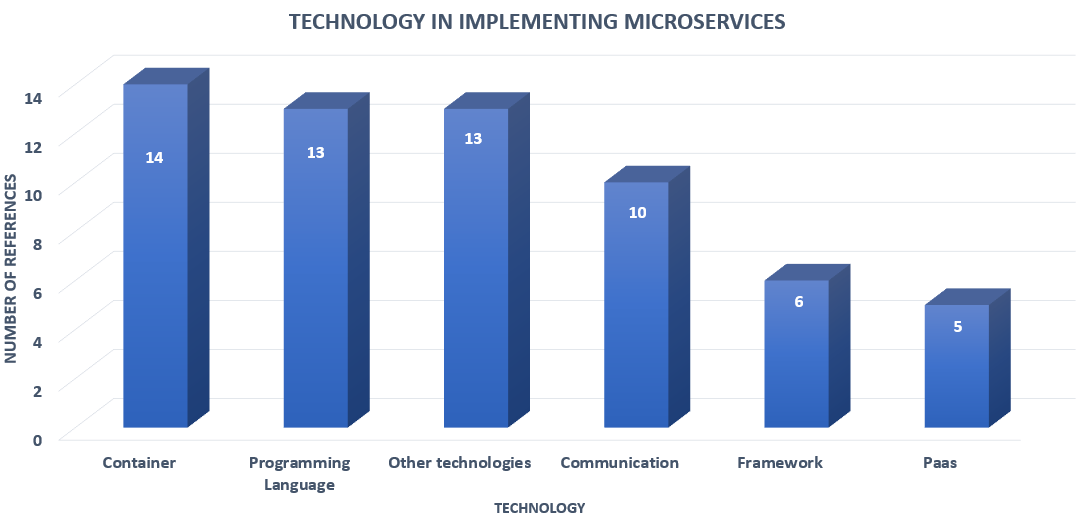
\includegraphics[width=0.5\linewidth]{images/commtechother.png}
	\caption{Technologies per group used for Implementing Microservices}
	\label{fig:tech-group}
\end{figure}	

In this section, we discuss RQ\#2, which is about the technologies used in the implementation of microservices according to our studied sources. Figure~\ref{fig:tech-group} shows the major groups of technologies that appeared in our studied references. We classified the technologies into \techgroupcount major groups.
Figure~\ref{fig:tech-distinct} shows the distinct technologies proposed to implement microservices. In total, we discovered \techcount different technologies in our data. 
The number of references of the groups showed in Figure~\ref{fig:tech-group} is the union of the references of the distinct technologies (Figure~\ref{fig:tech-distinct}) we classified in each group.  

\begin{figure*}[t]
	\centering
	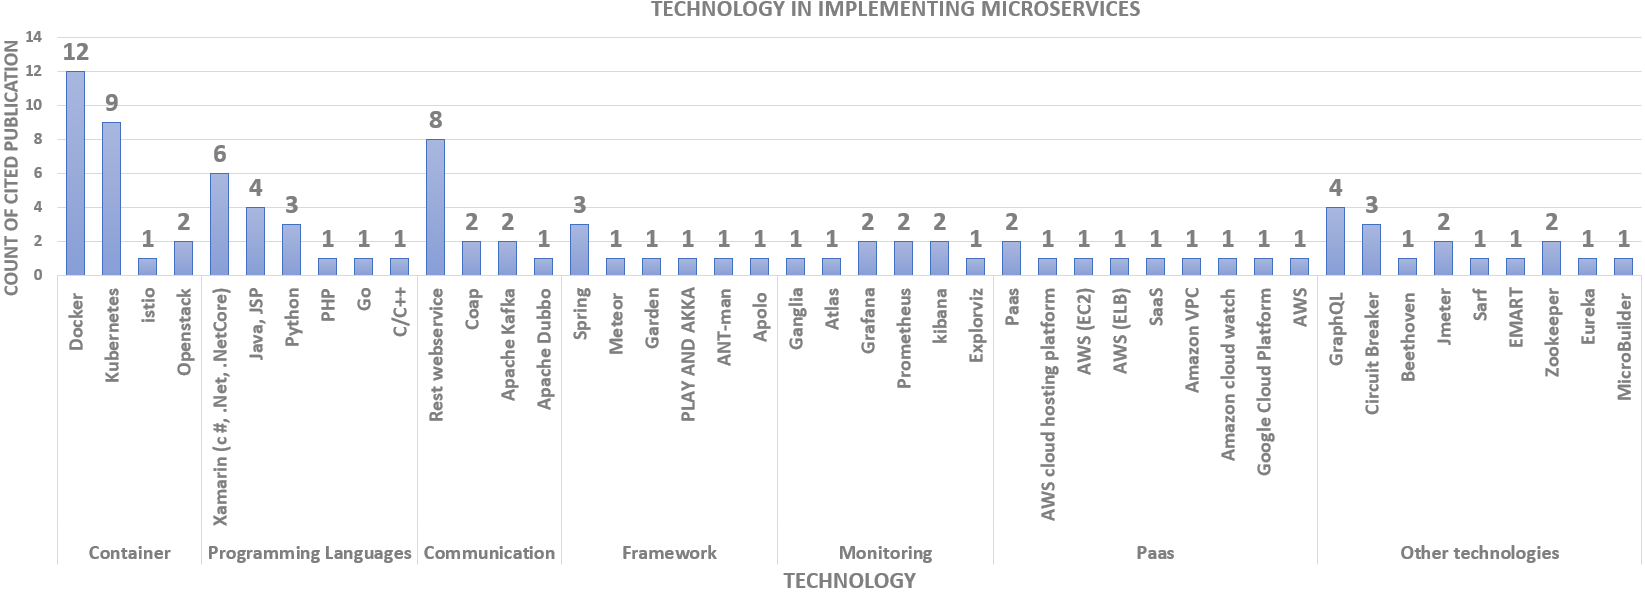
\includegraphics[width=\linewidth]{images/commontechupdated.png}
	\caption{Technologies in implementing microservices }
	\label{fig:tech-distinct}
\end{figure*}


\subsubsection{Containers}
Containers encapsulate discrete components of application logic provisioned only with the minimal resources needed to do their job. Containers and microservices enable developers to build and manage self-healing microservice-based applications more easily.
 
\par Docker: Docker is a platform for developing, shipping, and running applications. Developers can implement applications very fast by using docker~\cite{Sharaf2019, Kristiani2020, khan2020}. Moreover, it is simpler to create required services separately and manage them as microservices without affecting other services~\cite{leo2019, Hou2020, Kalske2017, Bahadori2018}. We can create a docker image for service and by running some docker commands, we can view our microservice application inside a docker container. Docker swarm applications can be deployed as services in a swarm cluster~\cite{Falatiuk2019, Venugopal2017, coulson2020}.
	
\par Kubernetes: Kubernetes is a container orchestration system that is well-suited to automate the management, scaling, and deploying of microservice applications~\cite{Zaytev2018, Kristiani2020, khan2020}. 
It is also possible to run kubernetes locally using MiniKube~\cite{leo2019, Kalske2017}.
Kubernetes ensures that the desired state (i.e., the state that we want the system to be in) and the actual state (i.e., the state that the system is actually in) are always in sync. Kubernetes continuously monitors the health of the cluster and ensures that the system is self-healing~\cite{Bahadori2018, Falatiuk2019, Venugopal2017}.

\par OpenShift: Red hat openshift is an open-source container application platform based on the kubernetes container orchestrator for enterprise application development and deployment~\cite{Johansson2019, Bahadori2018}.


\subsubsection{Programming Language}
When it comes to microservices development, a natural question is what language to choose. Developers have many options regarding programming languages to develop microservices. The programming languages mentioned in the citations are shown below.

\par Xamarin (C\#, .net, .netcore): asp.net, the web framework for .net, makes it easy to create the application programming interface to become microservices. Asp.net comes with built-in support for developing and deploying your microservices using docker containers~\cite{liu2018, chauvel2018, haugeland2020, Johansson2019, neves2019, Falatiuk2019}.

\par JAVA (Java, jsp): WSO2MicroservicesFramework for java has been used in implementing microservices~\cite{Sharaf2019, khan2020, KalskeM2017, Venugopal2017}.

\par Python: Python programming language uses flask application for building microservices~\cite{Ghebremicael2017, khan2020, Hou2020}.

\par PHP: PHP is also another programming language that can be used for implementing microservices~\cite{McElhiney2018}.

\par Go: Golang, also known as 'go' is popular for its concurrency and application programming interface support in terms of microservices architecture. It can be a good choice for microservices development. ~\cite{liu2018}.

\par C/C++: C++ is a programming language with imperative and object-oriented features that help developers write fast, portable programs. C++ is especially popular in areas where performance is crucial. Also, the compilation time and execution time of c++ is much faster than most other programming languages~\cite{Ghebremicael2017}. 


\subsubsection{Communication}

The goal of the microservice architecture is to create loosely coupled services, and communication plays a key role in achieving that. Therefore, services must interact using interprocess communication protocols such as http, amqp, or a binary protocol like transmission control protocol (TCP), depending on the nature of each service. Below we present the communication protocols used in the studied publications and grey literature.

\par REST API: REST API stands for 'representational state transfer' and It is a set of rules that developers follow when they create their application programming interface~\cite{Ndungu2019, Zhang2019}. One of the rules states that a user should be able to get a piece of data by using a specific URL~\cite{Koschel2017, Branko2018}. Microservices function as the building blocks of the application by performing various services, while restful application programming interface function as the communication that integrates the microservices into an application.\cite{liu2018, Zaytev2018, chauvel2018, Johansson2019}.

\par CoAP: CoAP and http are both based on the rest model and can be used as communication protocols to expose restful Web Services in a mobile device cloud. We will compare coap with http to better explain it. coap is a restful web transfer protocol optimized for communication between resource-constrained networks and nodes. CoAP uses the User datagram protocol (UDP) as its transport protocol, unlike http which operates on top of the reliable transmission control protocol and can be too complex for constrained environments. CoAP is not a blind compressed version of http, but a subset of rest common, with support of uniform resource identifier (URI) and http verbs, that gear towards machine-to-machine applications, hence it is an effective protocol for micro-services hosted on mobile devices~\cite{liu2018, khan2017}.

\par Apache Kafka: Apache kafka is an open-source distributed event streaming platform. Apache kafka is a powerful instrument for microservice architectures, which solves a variety of problems such as low-latency ingestion of large amounts of event data~\cite{wang2020, ebay}.

\par Apache Dubbo: Apache dubbo is a remote procedure call or remote procedure control-based service framework for programming. Dubbo is also a service governance framework, which provides service governance solutions such as service discovery and traffic scheduling for distributed microservices~\cite{Zhang2019}


\subsubsection{Framework}

Microservices can be implemented with a plethora of frameworks and using frameworks can help speed up the development of microservices. Below we present the frameworks used in implementing microservices in the analyzed references.

\par Spring framework: Spring is an open-source framework based on the java platform. Spring boot is part of the spring framework family to fastly create stand-alone applications. The distributed nature of microservices brings challenges. Spring helps us mitigate these. With several ready-to-run cloud patterns, spring cloud can help with service discovery, load-balancing, circuit-breaking, distributed tracing, and monitoring. It can even act as an application programming interface gateway ~\cite{KalskeM2017, selmadji2020, Santos2020}.

\par Meteor framework: Meteor is a framework meant to facilitate the whole web application development, encompassing the frontend, backend, as well as database. As such, it can be considered a full-stack web application framework. Meteor is written in javascript and is based on Node.js. The concept of having a proper microservices architecture using multiple meteor applications should be achieved reliably ~\cite{Tuuli2020}.


\par Apollo framework: Apollo is a great fit with microservice architectures and modern user interface frameworks like React. It serves as an abstraction layer that decouples services and applications so that each can be developed independently of the other, in any language and on any platform ~\cite{Kevin2015}.

\par Garden framework: Garden framework works like a spinnaker for implementing microservices~\cite{Ellen2018}.

\par ANT-man framework: an auto, native and transparent power management framework that can exploit fine-grained microservice variability for system efficiency\cite{Hou2020}.


\subsubsection{Monitoring}
Monitoring is a process of reporting, gathering and storing data. Some of the technologies/tools which are discussed before for monitoring microservices. 
\par Ganglia: Ganglia is one of the distributed monitoring tools for high-performance computing systems~\cite{Kristiani2020}.

\par Atlas: Atlas is a cloud monitoring tool which is newly introduced by netflix~\cite{Netflix}.

\par Explorviz: Explorviz is a monitoring and visualization approach, which uses dynamic analysis techniques to provide a live trace visualization of large software landscapes\cite{Lenga2019}.

\par Play AND Akka: The play framework is a web framework for the java virtual machine (JVM) that breaks away from the servlet specification. Play embraces a fully reactive programming model through the use of futures for asynchronous programming, work stealing for maximizing available threads, and akka for distribution of work. They are useful in building individual services, and leveraging both http and kafka for inter-service communication~\cite{khan2017}.

\par Grafana: Grafana is an open-source platform for data visualization, monitoring and analysis~\cite{KalskeM2017,Kalske2017}. 

\par Prometheus: Prometheus is an open-source monitoring system with a dimensional data model, flexible query language, efficient time series database and modern alerting approach~\cite{KalskeM2017, Kalske2017} 

\par Kibana: Kibana is a free and open user interface that lets us visualize your elasticsearch data and navigate the Elastic Stack~\cite{KalskeM2017, Kalske2017} 


\subsubsection{Platform as a Service (PaaS)}

Running microservices on a platform as a service fabric decreases solution fragility, reduces operational burden, and enhances developer productivity~\cite{rosa2018, Mikail2020}.

\par Amazon web services (AWS) cloud hosting platform: Among the primary benefits of a microservices architecture are the utilization and cost benefits associated with deploying and scaling components individually. While these benefits would still be present to some extent with on-premises infrastructure, the combination of small, independently scalable components coupled with on-demand, pay-per-use infrastructure is where real cost optimizations can be found~\cite{McElhiney2018}.

\par AWS auto-scaling group (EC2): Amazon elastic compute cloud is a part of amazon cloud-computing platform, amazon web services, that allows users to rent virtual computers on which to run their computer applications~\cite{McElhiney2018}.

\par Amazon AWS elastic load balancer: Elastic load balancing automatically distributes incoming application traffic across multiple targets~\cite{McElhiney2018}.

\par Software as a service (SaaS): Microservices are the resulting standalone services after breaking a software application down into separate components that perform their functions without being embedded in the application itself. Microservices are perfectly suited for saas, where each service is assumed to be part of a larger system~\cite{haugeland2020}.

\par Amazon VPC: Amazon virtual private cloud (Amazon VPC) is a service that lets us launch aws resources in a logically isolated virtual network that we define. Amazon~\cite{Amazon} uses amazon vpc to secure the traffic across cloud.

\par AWS Lamdba: AWS lamdba is a compute service that lets us run code without provisioning or managing servers. Lambda runs the code only when needed and scales automatically. AWS lambda is used to reduce infrastructure costs~\cite{villamizar2017}.

\subsubsection{Other Technologies}

\par GraphQL: Graph query language (GraphQL) is considered as an alternative for Representational state transfer application programming interface. It is most useful when it is able to combine different data sources into one and serve that up as one unified application programming interface. GraphQL hides the fact that we have a microservice architecture from the clients. From a backend perspective, we want to split everything into microservices, but from a frontend perspective, we would like all our data to come from a single application programming interface. Using graphgl is the best way that lets us do both~\cite{Ghebremicael2017, wang2020, overeem2018, gozneli2020}.

\par Circuit breaker: Hystrix, circuit breaker pattern allows us to build a fault-tolerant and resilient system that can survive gracefully when key services are either unavailable or have high latency \cite{Kalske2017}, \cite{Rodrigue2016}, \cite{Uber}. 

\par Beethoven: Beethoven is a platform composed of a reference architecture and a domain-specific language for expressing microservice communication flows~\cite{Monteiro2020}.

\par Apache JMeter: Apache jmeter is an apache project that can be used as a load testing tool for analyzing and measuring the performance of a variety of services. It is also used for performance-test in the microservice applications ~\cite{Hou2019}~\cite{Johansson2019}.

\par SArF : SArF is an sofware clustering algorithm and it has two characteristics. First, sarf eliminates the need of the omnipresent-module-removing step which requires human interactions. Second, the objective of sarf is to gather relevant software features or functionalities into a cluster. Thus, it is used to find the candidates for microservice from the source code ~\cite{Kamimura2018}.

\par EMART: Enhanced microservice adaptive reliability testing (EMART) is a tool for testing the applications~\cite{Russo2020}

\par Apache Zookeeper: Apache zookeeper is an open-source server for highly reliable distributed coordination of cloud applications. However, this architecture makes it hard to scale out to huge numbers of clients. ZooKeeper node called an 'observer' which helps address this problem and further improves zooKeeper's scalability~\cite{Kalske2017, KalskeM2017}.


\par Eureka Server: Eureka server is an application that holds the information about all client-service applications. Every micro service will register into the eureka server and Eureka server knows all the client applications running on each port and internet protocol address~\cite{Uber}.


\par MicroBuilder: MicroBuilder is the tool used for the specification of software architecture that follows representational state transfer microservice design principles~\cite{Branko2018} 




%% !TEX root = ../2021_microservices_wileytemplate.tex

\section{Discussion}\label{sec:discussion}

In this section, we describe the possible solutions we encountered for the top-10 challenges. Whenever possible, we also link the technologies we presented to the appropriate challenge. Therefore, we discuss the links between the presented results from our two research questions (Sections~\ref{sec:results-rq1} and~\ref{sec:results-rq2}), focusing on how to address the challenges, i.e., we show the challenges we encountered and discuss the solutions and technologies used to address the top-10 challenges.

\subsection{Migration}%#1

Before splitting or migrating the application into multiple services we need to understand its scope and architecture. Components that are used by most users should be considered first for migration. 
%
We can employ the SArF method based on clustering to identify candidates in the source code to be turned into microservices. The method also visualizes the extracted candidates to show the relationship between them and the overall structure. The candidates and visualization help the developers to capture the overview of the whole system.\cite{Kamimura2018}

In database migration, MongoDB and Meteor Framework, both provided tools for updating the upcoming migration host. Public clouds offer many services that help with the goals of this optimization, which makes it a logical choice to migrate the application hosting server onto a Cloud Service Provider (CSP).\cite{Tuuli2020} %Also, GCP offers its Kubernetes as a service (GKE) as part of its services. It was suitable as the target destination for the application containers~\cite{haugeland2020}.

%Migration triggers are handled by different strategies as follows~\cite{overeem2018}:
%(i) change of model by modeler - all existing models could be changed instead of a single model;
%(ii) change to the transformation environment - updated packages need to be redeployed to upgrade the instances;
%and (iii) change to the runtime environment - the application needs to be migrated and then Incremental migration. 

There are some practices to aid the migration process.
For instance, service identification where we analyze artifacts (e.g., source code, documentation) from the monolithic application to decide the corresponding microservices.
%
Another practice is packaging the microservice where the transformations are to be performed on the source code.\cite{selmadji2020}
%
Many organizations consider a gradual process of moving to the cloud with hybrid cloud architecture.\cite{Mikail2020}
%  \item For managing common code, the study enumerated several options employed by the participants. While most participants rely on promises and challenges of Microservices~\cite{wang2020}, an exploratory study shared libraries which are the emerging sidecar technology could be a promising and elegant microservice-native solution to this problem. 
Numerous options for managing the application programming interface (API) are there. The API gateways and client libraries, although not adopted by most of the practitioners and have a high potential to mitigate the burden related to managing API changes.\cite{wang2020}
%  \item Options for supporting product variants are there. Each of these solutions has advantages and disadvantages, with most practitioners applying a role-based access model to support different product offerings within the same code base. 


\subsection{Performance}%#2
The increase in resource usage may cause a microservices-based application to execute slower. We can overcome this challenge by introducing additional servers. Logs can help identify bottlenecks, as we can log performance data and detect the problems. %We should take advantage of logging to store performance data in a repository so that we can analyze the data at a later point in time. 
We can implement throttling, handle service timeouts, implement dedicated thread pools, implement circuit breakers and take advantage of asynchronous programming to boost the performance of microservice-based applications.\cite{Ghebremicael2017, Johansson2019, Zhihui2020}

Apache JMeter can be used to performance-test our microservice applications. Microservice criticality factor metric (MCF) to measure the overall impact of performance scaling on a microservice from the whole application's perspective.\cite{Hou2019} Beethoven (a platform composed of a reference architecture) could be used to measure and increase the performance of microservices.\cite{Monteiro2020}


\subsection{Scalability}%#3
 To scale successfully, each microservice needs to scale both individually, and as part of a larger system. Doing so requires that the dependencies of each microsystem also to scale with it. We can containerize and manage  microservices using Docker or Kubernetes.\cite{coulson2020, khan2020, McElhiney2018, Bahadori2018}


\subsection{Testing}%#4
The best approach to solving testing challenges is adopting various testing methodologies, tools and leveraging continuous integration capabilities through automation.
Some of the options to consider are enhanced microservice adaptive reliability testing (EMART),\cite{Russo2020} Apache Jmeter,\cite{Johansson2019} testing as a service,\cite{Vanska2019} integration testing, test doubles,\cite{Huttunen2017} end-to-end testing, and a/b testing.\cite{Dmitrii2019, Zaytev2018} Good quality tooling is needed like chaos monkey which will do destructive testing in the production environment to understand the resilience of system.\cite{Netflix}


\subsection{Monitoring}%#5
We can monitor microservices by using open-source tools like Prometheus with Grafana APIs by creating gauges and matrices, google cloud platform (GCP) Stackdriver, Kubernetes monitoring, and Amazon cloudwatch.\cite{Venugopal2017, Kalske2017paper, Zhang2019, Monterio2018}

Ganglia monitoring system is one of the distributed monitoring tools for high-performance computing systems.\cite{Kristiani2020} The proposed monitoring framework includes an integrated scheduling tool, data collector, big data storage, elastic scaling manager.\cite{Zhihui2020} %For device failure detection in microservices kieker trace analysis tool is used to analyze the application and the trace tool used for visualizing are graphViz, gnuplotzunit~\cite{Saman2017}.
%
%The conceptual model of a dashboard for monitoring is proposed and this model consists of components, the interaction between components, and the requirements for each component.
%
A black-box approach and monitoring of the microservices through its endpoint is done.\cite{Utomo2020} Spotify\cite{Kevin2015} and Netflix\cite{Netflix} employ their tools, Heroic and Atlas, for monitoring.

%ExplorViz uses kieker (dynamic analysis tool) to instrument software systems for a dynamical analysis of their runtime behavior~\cite{Lenga2019}. Instead of using kieker’s analysis methods, explorviz uses its own and instructs kieker to send the gathered monitoring data called records. The Analysis service creates traces from these records which are sent to the Landscape service which creates the models which are visualized in the frontend service of explorViz. The assessment confirmed that one of the central prerequisites for the effective usage of explorViz is a thorough prior knowledge of the entire monolithic architecture. The evaluation also demonstrated that finding a suitable division into self-contained systems or microservices is a highly complex process that requires experience and time.


\subsection{Security}%#6
The first step to a secure solution based on microservices is to ensure security which should be included in the design. Some fundamental tenets\cite{Olaf2016} for all designs are: 
(i) encrypt all communications (using https or transport layer security); 
(ii) authenticate all access requests;
(iii) do not hard code certificates, passwords, or any form of secrets within the code;
(iv) use devsecops tools designed for microservice architecture environments to scan code as it is developed;
and (v) define the APIs and strictly make sure all communications comply.

In a typical microservices architecture, communication between the services can be in the same or different machines or even between different data centers. Due to this complexity in the communication, security in a microservices-based application is important to authorize access to a protected resource.
In a monolith, the facade pattern aggregates the data that is retrieved from multiple services. On the contrary, in a microservices-based application, the API Gateway is used for the same purpose. The API Gateway pattern can be used in a microservices-based application to secure access to the microservices by abstracting the underlying microservices from external clients. The other strategies that are adopted include implementation of ssl, oauth, and containerization.\cite{Zaytev2018, Monterio2018, tenev2019}
%
Some of the best practices in securing microservices are building security from the start, deploying security at container level, multifactor authentication, user identity and access tokens such as oauth 2.0 and openid.\cite{Gonchar2017} Amazon~\cite{Amazon} uses amazon vpc to secure the traffic across cloud.


\subsection{Cost}%#7
Cost could be an significant factor when building microservices~\cite{Michael2018, Netflix, Koschel2017}. 
%
Adopting a microservices architecture quickly defray those costs by returning large amounts of business and technical value~\cite{Leo2019, McElhiney2018}. A microservice architecture, with fewer application dependencies and simple APIs will immediately reduce the time and money spent on application maintenance. Savings on application maintenance have shown to be more than enough to cover the initial costs within a few years.\cite{Otharson2019} 
A good set of guidelines and practices at the company level is needed. After the load was removed, the instances should be terminated automatically by aws to save cost.\cite{McElhiney2018} 

%Testing the off-the-shelf hardware to reduce hardware costs. Invest in the team to create white box solutions that focused on reducing costs, using a reference architecture. AWS Lambda functions can be triggered based on events ingested into amazon sqs queues, s3 buckets where aws manages the polling infrastructure on our behalf with no additional cost\cite{Ndungu2019, Zhang2019, Koschel2017}. The use of services specifically designed to deploy and scale microservices, such as aws lambda is used to reduce infrastructure costs by 70\% and Microservice implemented with play reduce up to 13\% cost~\cite{villamizar2017}.

\subsection{Complexity}%#8
Microservices architecture can be more complex than legacy applications. To handle this complexity and reduce the risks involved, we should use the right tools and technologies in place.
%Complexity can be addressed for each and every situation.
If the complexity is based on integrating the legacy and internal system on the cloud services then we can use the Platform as a Service (PaaS) model.\cite{rosa2018} When the applications are moving on-premise to Software as a Service (SaaS), directly changing the code is not feasible because many customers share one instance of an application code.
%
Chauvel and Solberg\cite{chauvel2018} propose an approach to enable deep customization on multi-tenant SaaS using intrusive microservices.

Another possible solution is adding a service mesh to microservices that can improve visibility, monitoring, management, and security.\cite{Zaytev2018, Ndungu2019} A service mesh allows developers to make changes without touching the application code itself. It provides the ability to mirror and monitor traffic on multiple versions of the same service, which lets developers test capabilities before deployment and determine the best way to route traffic through the system for specific types of use patterns.\cite{gozneli2020,Premchand2018}

%MicroBuilder is the tool used for the specification of software architecture that follows REST microservice design principles. MicroBuilder comprises MicroDSL and MicroGenerator modules. The MicroDSL module provides the MicroDSL domain-specific language used for the specification of microservice architecture~\cite{Branko2018}.


\subsection{Decomposition}%#9

In transitioning an existing monolith to a microservices, we would typically need to decompose the existing application into granular microservices.\cite{Taibi2019} During this transitioning process, we would typically need to decompose the monolith to building more and more granular microservices to suit the business needs. Once this is accomplished, there would be more moving parts in the application.\cite{Carvalho2019} As a result, this would lead to operational and infrastructural overheads, i.e., configuration management, security, provisioning, integration, deployment, monitoring, etc. One way to reduce these complexities is by using containerization. In using containerization, provisioning, configuration, and deployment of microservices would be simplified.\cite{Zhang2019}

To define the functional scope of microservices many authors propose using domain-driven design.\cite{Merson2020, neves2019, Zrzavy2020}
The key concepts of domain-driven design that helps in defining scopes are:
(i) analyze domain;
(ii) define bounded context;
(iii) define entities, aggregates, and services;
and (iv) finally identify microservices. 

%A service can have the scope of microservice. Microservice can have the scope of a bounded context. For inter-microservice interaction, we can use domain events with asynchronous messaging API calls, and service data replication.

Some factors must be considered when defining the size of a microservice and when we are defining a microservice granularity. Moreover, more factors must be considered to achieve a successful implementation and performance.
The most important point is balancing. Although we may consider different factors to define the level of granularity, the key purpose is to analyze all the applicable criteria and to evaluate the possible tradeoffs that will have to be made in this process. Key points to consider are:\cite{Yan2020}
(i) get a clear picture of the solution architecture;
(ii) functional decomposition patterns must be applied, this helps in defining services and splitting them;
and (iii) separate reusable activities into reusable services.
%
To achieve the above, the key technologies used were service registration and discovery, remote service calling, circuit-breaker mechanism, service link tracking, and annotation interfaces.


\subsection{Integrating}%#10
Integration of APIs, services, data, and systems has been a challenging yet essential requirement in the context of enterprise software application development. %Before integrating all of these disparate applications in point-to-point style was done, which was later replaced by the enterprise service bus (ESB) style, alongside the service oriented architecture (SOA).
Integration Platform as a Service (iPaaS) provides a platform in the cloud to support the application, data, and system-to-system integrations, using a mix of cloud services, mobile apps, on-premises systems, and internet of things integrations. 
%
%A message-Oriented middleware services (momPaaS) was proposed to support the communication and integration between the different microservices implemented in the respective system, thus supporting the message exchange with different protocols.
%Enterprise horizontal portal services (Portal PaaS) can be used to provide a B2B portal that is integrated with the microservices layer.
Integration platform services (iPaaS) was recommended for situations when the integration and exchange of information between cloud applications and on-premise and legacy applications are required.\cite{rosa2018}

Architecture style makes it possible to achieve fine-grained incremental migration. The integration of this architecture style manifests itself in two ways. First of all, the runtime environment should be able to host distributed microservices. The benefits of this are an improved upgradability, scalability, resilience, and resource sharing.
Second, the transformation environment should consist of independent microservices. This enables the incremental transformation of the model through the pattern incrementality by traceability.\cite{overeem2018, liu2018}

Continuous integration and continuous delivery both go hand in hand with microservices. Without these two practices, it becomes very hard to handle multiple services, their deployments, and validating the actions of the service.\cite{Kalske2017paper, Zhang2019} 







%% !TEX root = ../final_paper.tex

\section{Threats to validity}\label{sec:threats}
In this section we acknowledge the threats to validity in the process we use in our systematic
literature review. We discuss each threat and its mitigation strategy based on the guidelines presented by Kitchenham and Charters~\cite{Kitchenham2007}.


\par \textit{Construct validity:} 
Construct validity concentrates on the sufficiency of the study's design to address the research questions. Many trials and discussions were carried out to define a search string and mitigate any subjectiveness in our study. The search string that resulted in the most relative number of results was selected. To mitigate threats related to the study selection strategy, the strategy was based on the software engineering systematic review guidelines presented by Kitchenham et al~\cite{kitchenham2015}.
%\keerthana{i cited kitchenham 2015 because it has construct validity in page 25,35}

 
\par \textit{Internal validity:} 
Internal validity is concerned with the conduct of the study. To mitigate internal validity threats during the study selection process, we followed the guidelines presented by Kitchenham and Charters~\cite{Kitchenham2007} to construct the search strategy and prevent any systematic error.
The procedure and its implementation were discussed by the main author and the supervisor to mitigate any subjectiveness in our study. The research questions we defined helped in selecting relevant studies. However, the chosen inclusion and exclusion criteria might have led to missing contributions that could have inspired the microservices field. While extracting videos for inclusion in the study results, we tried to include videos as much as we could using the search keywords the author might have mentioned during his presentation. We mitigated this threat by having two persons (the main author and the supervisor) going over the selection process separately. Moreover, if one person involved voted to include a reference, it was included. Therefore, any subjective bias on the inclusion or exclusion of references was lessened. 
%\henrique{According to Kitchenham2007, which you explicitly stated to be using at the begging of the section, internal validity is "The extent to which the design and conduct of the study are likely to prevent systematic error". I do not see how your text fits into that definition. Your text is about possible missed contributions. I think you are on the right path but missed the mark. You will need to shift the tone of your text for internal. Remember the goal here is 'prevent systematic error'. Your threat for construct validity is more in tune with the internal according to Kitchenham (avoiding bias in the conduct/design is important to prevent a systematic error in the study).}
%\keerthana{rewritten the whole paragraph above}

\par \textit{External validity:}
External validity is concerned with the generalizability of a study’s
findings~\cite{Kitchenham2007}. Since our primary studies are obtained from a large extent of online sources, our results and observations may be only partly applicable to the broad area of practices and general disciplines of microservices. Hence to mitigate this threat we performed multiple iterations of backward snowballing to expand the search scope.
%\henrique{First, it is almost impossible to eliminate an external threat. You are too ambitious. At most, you can claim to mitigate an external threat. Second, I am almost certain we did not perform a forward snowballing. We did an "informal" backward snowballing at the first stage of the SLR. It is misleading to claim we perform snowballing at other stages or that this snowballing at the first stage is responsible to mitigate such a threat. }
Though the aim was to
cover a representative body of implementation and challenges of microservices prioritization literature, the findings may not have prioritized specific challenges or implementation technologies outside of the primary studies. 
%Im trying to say is that the technology and challenges might be only limited to the collected primary studies
Moreover, there is a risk of having missed relevant industrial studies, because concepts related to those included in our search strings are differently named in such studies (e.g., a study discussing architecture of microservices may not employ the terms “challenges” but rather some synonyms). To mitigate this threat to validity, we have explicitly included all relevant synonyms in our search strings by looking at results for every iteration of chosen search string and finding enough articles to address the research questions. 
%this is where we had a back and forth mails to discuss upon the most relevant search string.
%\henrique{Once again I think you have the right idea and path for this threat but the wrong execution. External validity is to generalize our results. The problem with SLR to generalize content is that our selection could not represent the actual reality.}


\par \textit{Conclusion validity:} 
Threats to conclusion validity are related to issues that affect the ability to draw the correct conclusions from the study \cite{Kitchenham2007}. From the reviewers’ perspective, a potential threat to conclusion validity is the reliability of the data extraction categories from the selected sources. The technologies and challenges collected during the systematic literature review might be limited to the collected evidence. We are aware that the microservices challenges could be addressed by a wide range of solutions but we have answered according to the solutions we could find using the studied references. Although we did not explicitly address this threat, we claim it was mitigated due to the heterogeneity of the references we used. Additionally, to ensure validity multiple sources of data were analyzed, i.e., articles, blogs, news, and videos. %Furthermore, in the event of a disagreement between the one reviewer, the second reviewer acted as an arbitrator to ensure the agreement was reached.



%% !TEX root = ../2021_microservices_wileytemplate.tex

\section{Related Work}\label{sec:related-work}

Motivated by discipline of microservices, several studies have been conducted to examine the existing literature in the field. Some of the studies on microservices are discussed in this section.
%
An interesting systematic literature review by Ghani et al.~\cite{Ghani2019} focuses on the testing challenges and quality-related aspects concerning testing. They also provide some solutions for the issues with testing. We decided to have a more broad overview of all the challenges instead of focusing on just one. Although, we did find that testing is one of the most cited challenges in our studied literature. 
%Moreover, there is a claim that their study criteria are biased during the selection of primary study and analysis

Francesco et al.~\cite{Francesco2019} motivation are on the publication trends of architecting microservices and the focus of architecting with microservices. One of their research questions is similar to our research question about the potential for industrial adoption of existing research on architecture with microservices. However, this is again focused on industrial needs whereas our study consists of a broader scope with both practitioner and academic material.
%
Pahl and Jamshidi~\cite{Claus2016} conducted a systematic mapping on microservices and it is the classification of research directions in the field and highlights the perspectives considered by researchers.

We also analyzed two survey studies.
Dragoni et al.~\cite{Dragoni2017} performed a survey on microservices. The survey gives an overview of software architecture, mostly providing the reader with references to the literature, and guiding the readers in the itinerary towards the advent of services and microservices. We focus on the adoption and implementation of microservices. We followed a systematic literature review method which is easier to reproduce.
%
Ghofrani et al ~\cite{ghofrani2018} study are similar to finding the challenges in adopting microservices but limited to survey conducted to the industrial peers. They do provide solutions from the experts to improve the aspects of the architecture. Although, it focuses on only artifacts from third parties, and not all challenges are addressed by the authors. Only the challenges faced in that company are considered by them.


% !TEX root = ../2021_microservices_wileytemplate.tex

\section{Conclusion}\label{sec:conclusion}

In this paper, we reported the results of our systematic literature review in microservices. We collected and read a total of 81 references from both scientific and grey literature sources we deemed relevant to answer our research questions. Our work can be used as groundwork and complementary to the existing literature reviews to guide researchers to open issues and challenges in microservices and offer an overview of solutions to consider.

The first research question addresses the challenges in adopting microservices. Among the collected publications, we identified \challengecount different challenges. The most mentioned challenges were migration (14 references), performance (11 references), scalability (10 references), and testing (10 references). The least mentioned were power management (2 references) and load balancing (2 references). 

The second question addresses the technologies used in implementing microservices. We distinguished a total of \techcount reported technologies which we grouped into the following categories: container, programming languages, other technologies, communication, framework, and platform as a service. The most mentioned technology categories were Container (14 references), programming languages (13 references). Other technologies also have many references to be top-ranked (13 references), however, it is a miscellaneous category with unrelated technologies. When we look at the ungrouped technologies, the most cited are Docker (12 references), Kubernetes (9 references), and REST (8 references).

We also discussed the possible solutions for each of the challenges. The solutions may vary based upon the requirement and necessity of adoption of microservices. According to the gathered solution, a necessary aspect to remember is to analyze the entire system before migrating to microservices.

Future work includes (i) adding more grey literature and valuable resources; (ii) conducting a survey with the industrial peers; and (iii) providing some broader scope to the collected materials about the aspects and architecture of microservices.









%\nocite{*}% Show all bib entries - both cited and uncited; comment this line to view only cited bib entries;
\bibliography{wileyNJD-AMA} %BST file for AMA reference style
%\bibliography{wileyNJD-APA} %BST file for APA reference style
%\bibliography{wileyNJD-AMS} %BST file for AMS reference style
%\bibliography{wileyNJD-VANCOUVER} %BST file for Vancouver reference style


%\bibliography{final_paper_bibliography}


%\section*{Author Biography}

%\begin{biography}{\includegraphics[width=66pt,height=86pt,draft]{empty}}{\textbf{Author Name.} This is sample author biography text this is sample author biography text this is sample author biography text this is sample author biography text this is sample author biography text this is sample author biography text this is sample author biography text this is sample author biography text this is sample author biography text this is sample author biography text this is sample author biography text this is sample author biography text this is sample author biography text this is sample author biography text this is sample author biography text this is sample author biography text this is sample author biography text this is sample author biography text this is sample author biography text this is sample author biography text this is sample author biography text.}
%\end{biography}

\end{document}
